\chapter{Symmetrie en puntgroepen}\label{ch:b3:point-groups}

Draai een sneeuwvlok over zestig graden en er verandert niets; draai een
benzeenmolecuul over dezelfde hoek, en zijn zes koolstofatomen en zes
waterstofatomen vallen precies op elkaars plaatsen. De symmetrie van een
molecuul bepaalt een aantal van zijn eigenschappen nog vóór elke
berekening: of het een dipoolmoment kan hebben, of het kan bestaan als twee
spiegelbeeldvormen, welke van zijn vibraties infraroodlicht absorberen,
welke orbitalen mogen mengen. Om haar te gebruiken, leenden chemici bij de
wiskunde de taal van de groepen. Dit hoofdstuk definieert de
\omterm{def:b3:point-groups:operation}{symmetrieoperaties} van een molecuul, brengt ze samen in zijn \omterm{def:b3:point-groups:point-group}{puntgroep},
geeft een procedure om die groep te vinden, bewijst twee stellingen over
polariteit en chiraliteit, en voert de karaktertabellen in waarop
\cref{ch:b3:group-theory-applied} voortbouwt.

\begin{recall}
Het deel van jaar~1 voorspelde de vorm van moleculen met het VSEPR-model,
definieerde het dipoolmoment van een polair molecuul, en definieerde
chiraliteit: een chiraal molecuul kan niet op zijn spiegelbeeld gelegd
worden. Het deel van jaar~2 gebruikte symmetrie in woorden om de
fragmentorbitalen van \ce{H2O} en \ce{NH3} op te bouwen.
\end{recall}

\begin{omfigure}
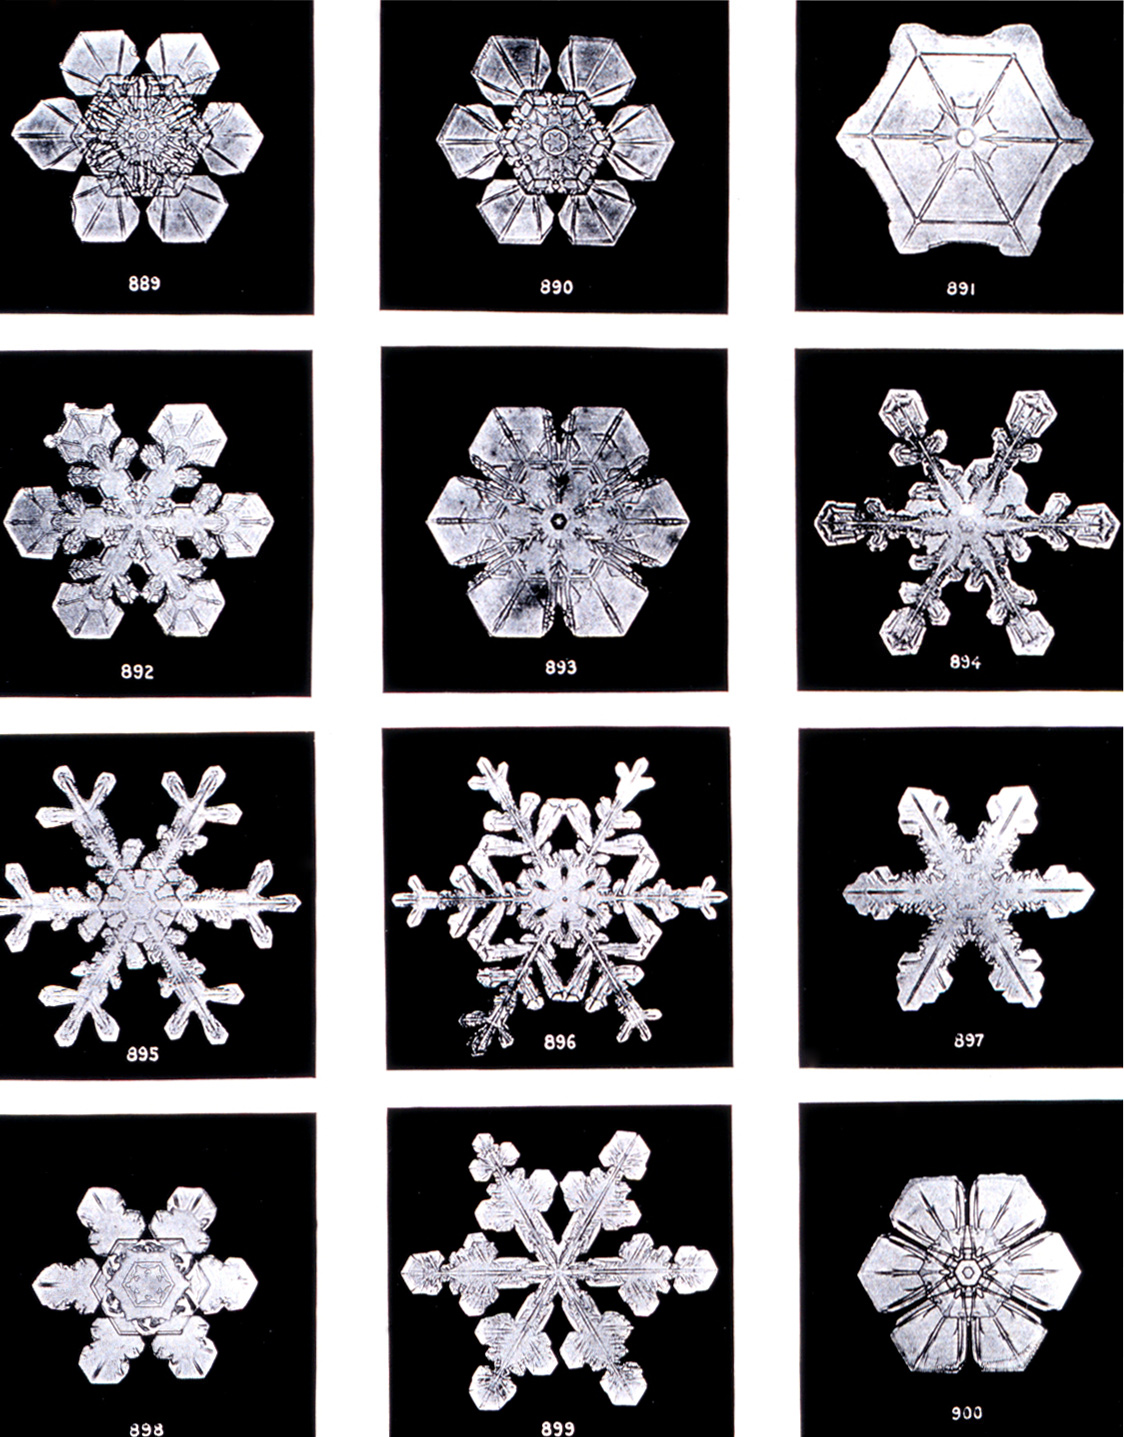
\includegraphics[width=0.4\linewidth]{images/book4/bentley-snowflakes.jpg}\hspace{1em}%
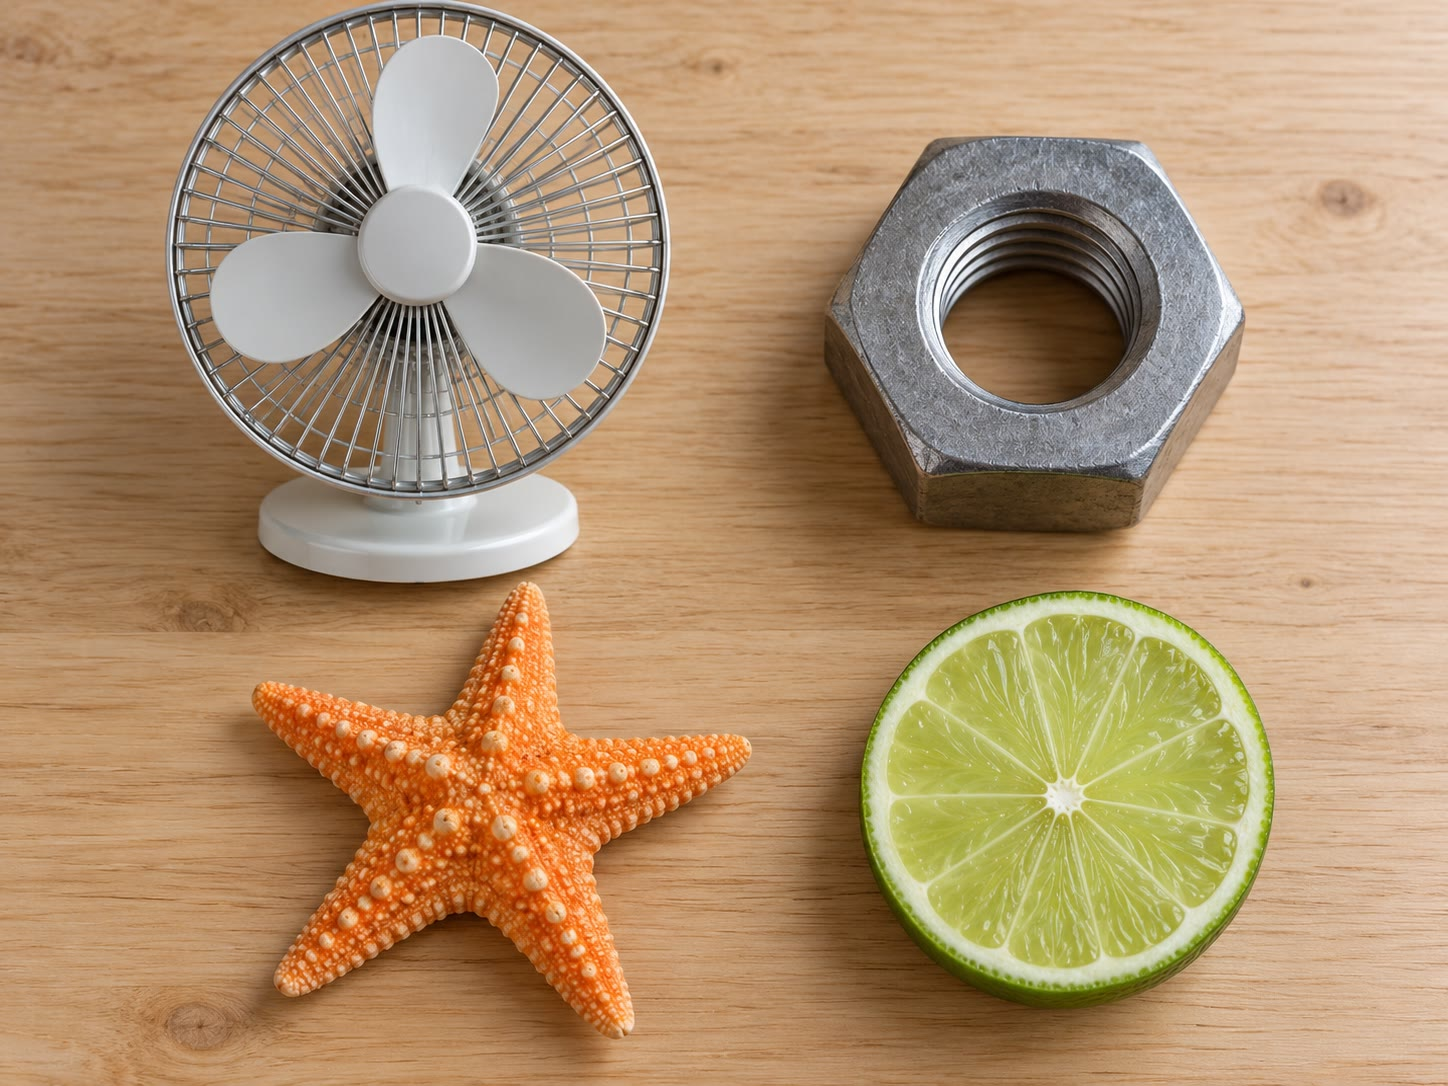
\includegraphics[width=0.48\linewidth]{images/book4/ai/b3-04-symmetric-objects.jpg}

{\small Links: sneeuwkristallen, gefotografeerd door Wilson Bentley rond
1902, elk met zesvoudige symmetrie. Rechts: alledaagse voorwerpen met
drievoudige, zesvoudige en vijfvoudige rotatiesymmetrie.}
\end{omfigure}

\section{Symmetrieoperaties en symmetrie-elementen}

\begin{definition}[Symmetrieoperatie, symmetrie-element]\label{def:b3:point-groups:operation}
Een \emph{symmetrieoperatie}\index{symmetrieoperatie} is een beweging of
spiegeling die een molecuul achterlaat in een configuratie die niet te
onderscheiden is van de oorspronkelijke (elk atoom op een positie die
eerder door een atoom van dezelfde soort bezet was). Een
\emph{symmetrie-element}\index{symmetrie-element} is het meetkundige
object --- een punt, een rechte, een vlak --- ten opzichte waarvan de
operatie uitgevoerd wordt.
\end{definition}

Elk molecuul heeft de identiteitsoperatie $E$, die niets doet. De andere
zijn er in vier soorten.

\begin{definition}[Eigenlijke rotatieas, hoofdas]\label{def:b3:point-groups:rotation}
Een \emph{eigenlijke rotatieas}\index{eigenlijke rotatieas} $C_n$ is een
rechte waarrond een rotatie over $2\pi/n$ een \omterm{def:b3:point-groups:operation}{symmetrieoperatie} is, ook
geschreven als
$C_n$; haar machten $C_n^k$ zijn rotaties over $2\pi k/n$, en $C_n^n = E$. De
as met de hoogste $n$ is de \emph{hoofdas}\index{hoofdas}, die als $z$-as
genomen wordt.
\end{definition}

\begin{definition}[Spiegelvlakken]\label{def:b3:point-groups:mirror}
Een \emph{spiegelvlak}\index{spiegelvlak} $\sigma$ is een vlak waarin
spiegeling een \omterm{def:b3:point-groups:operation}{symmetrieoperatie} is; $\sigma^2 = E$. Een spiegelvlak is een
\emph{verticaal spiegelvlak}\index{verticaal spiegelvlak} $\sigma_v$ als het
de \omterm{def:b3:point-groups:rotation}{hoofdas} bevat, een \emph{horizontaal
spiegelvlak}\index{horizontaal spiegelvlak} $\sigma_h$ als het er loodrecht
op staat, en een
\emph{diëdrisch spiegelvlak}\index{diedrisch spiegelvlak@diëdrisch spiegelvlak}
$\sigma_d$ als het de \omterm{def:b3:point-groups:rotation}{hoofdas} bevat en de hoek tussen twee
$C_2$-assen die er loodrecht op staan, middendoor deelt.
\end{definition}

\begin{definition}[Inversiecentrum]\label{def:b3:point-groups:inversion}
Een \emph{inversiecentrum}\index{inversiecentrum} $i$ is een punt
waardoor inversie, $(x, y, z) \mapsto (-x, -y, -z)$, een
\omterm{def:b3:point-groups:operation}{symmetrieoperatie} is.
\end{definition}

\begin{definition}[Oneigenlijke rotatieas]\label{def:b3:point-groups:improper}
Een \emph{oneigenlijke rotatieas}\index{oneigenlijke rotatieas} $S_n$ is een
rechte waarrond een rotatie over $2\pi/n$, gevolgd door een spiegeling in
het vlak loodrecht erop, een \omterm{def:b3:point-groups:operation}{symmetrieoperatie} is. $S_1 = \sigma$ en $S_2 = i$.
\end{definition}

\begin{example}[De elementen van vier moleculen]\label{ex:b3:point-groups:elements}
\ce{H2O}: $E$, een $C_2$-as die de hoek H--O--H middendoor deelt, en twee
verticale vlakken, het molecuulvlak en het vlak loodrecht daarop. \ce{NH3}:
$E$, een $C_3$ door N (operaties $C_3$ en $C_3^2$), en drie $\sigma_v$, elk
met één binding N--H. \ce{BF3}: een $C_3$, drie $C_2$ langs de bindingen
B--F, $\sigma_h$ (het molecuulvlak), drie $\sigma_v$, en een $S_3$. \ce{CH4}:
vier $C_3$ langs de bindingen C--H, drie $C_2$ die de hoeken H--C--H
middendoor delen en die ook $S_4$-assen zijn, en zes $\sigma_d$, elk met
twee bindingen C--H (figuur hieronder).
\end{example}

\begin{omfigure}
\begin{tikzpicture}[font=\small]
  % H2O, side view: molecular plane xz (shaded), C2 along z
  \begin{scope}
    \fill[omDef!10] (-1.5,-1.0) -- (1.5,-1.0) -- (1.5,1.2) -- (-1.5,1.2) -- cycle;
    \fill[omThm!12, opacity=0.8] (-0.45,-1.35) -- (0.45,-0.65) -- (0.45,1.55) -- (-0.45,0.85) -- cycle;
    \draw[densely dashed, black!70] (0,-1.4) -- (0,1.7) node[above] {$C_2$};
    \node[aO] (o) at (0,0.5) {};
    \node[aH] (h1) at (-0.95,-0.25) {};
    \node[aH] (h2) at (0.95,-0.25) {};
    \begin{scope}[on background layer]
      \draw[bond] (o.center) -- (h1.center) (o.center) -- (h2.center);
    \end{scope}
    \node[omDef, anchor=north west] at (-1.5,1.2) {$\sigma_v(xz)$};
    \node[omThm, anchor=west] at (0.5,-0.85) {$\sigma_v'(yz)$};
    \node[anchor=north] at (0,-1.6) {\ce{H2O}, $C_{2v}$};
  \end{scope}
  % NH3, top view along C3
  \begin{scope}[xshift=4.0cm]
    \foreach \a in {90,210,330}{\draw[ommirror] (0,0) -- (\a:1.35); \draw[ommirror, black!40] (0,0) -- (\a+180:1.0);}
    \foreach \a in {90,210,330}{\node[aH] at (\a:0.95) {};}
    \node[aN] at (0,0) {};
    \pic at (0,0) {omthreefold};
    \node[anchor=north] at (0,-1.6) {\ce{NH3}, $C_{3v}$ (van bovenaf)};
  \end{scope}
  % BF3, top view; sigma_h = plane of the paper (thick circle)
  \begin{scope}[xshift=8.0cm]
    \draw[ommirror] (0,0) circle (1.3);
    \foreach \a in {90,210,330}{\draw[ommirror] (\a:1.3) -- (\a+180:1.3);}
    \foreach \a in {90,210,330}{\pic[rotate=\a-90] at (\a:1.42) {omtwofold}; \pic[rotate=\a-90] at (\a+180:1.42) {omtwofold};}
    \foreach \a in {90,210,330}{\node[aF] at (\a:0.95) {};}
    \node[aX={pink!70!gray}{5.6mm}] at (0,0) {};
    \pic at (0,0) {omthreefold};
    \node[anchor=north] at (0,-1.6) {\ce{BF3}, $D_{3h}$ (van bovenaf)};
  \end{scope}
\end{tikzpicture}

{\small \omterm{def:b3:point-groups:operation}{Symmetrie-elementen}. \ce{H2O}: de $C_2$-as (gestreept) en twee
verticale spiegelvlakken. \ce{NH3} en \ce{BF3} gezien langs hun \omterm{def:b3:point-groups:rotation}{hoofdas}
(driehoekje): dikke lijnen zijn spiegelvlakken die op hun kant gezien
worden; in \ce{BF3} stelt de dikke cirkel het horizontale \omterm{def:b3:point-groups:mirror}{spiegelvlak} voor
(het vlak van de bladzijde) en de lensvormige tekens de drie $C_2$-assen
die erin liggen.}
\end{omfigure}

\section{Groepen}

\begin{proposition}[Producten van symmetrieoperaties]\label{prop:b3:point-groups:closure}
Twee \omterm{def:b3:point-groups:operation}{symmetrieoperaties} van een molecuul na elkaar uitvoeren levert
opnieuw een \omterm{def:b3:point-groups:operation}{symmetrieoperatie} van dat molecuul op. Samen met $E$ en de
inverse van elke operatie vormt de verzameling \omterm{def:b3:point-groups:operation}{symmetrieoperaties} een
groep: een associatief product, een identiteit, een inverse voor elk
element.
\end{proposition}

\begin{proof}
Elke operatie laat het molecuul ononderscheidbaar van zichzelf, dus twee
na elkaar ook. Het product van operaties (samenstelling van afbeeldingen
van de ruimte) is associatief; $E$ is de identiteit; een ongedaan gemaakte
operatie (een rotatie over de tegengestelde hoek, een herhaalde
spiegeling) is ook een \omterm{def:b3:point-groups:operation}{symmetrieoperatie}.
\end{proof}

\begin{proposition}[Een gemeenschappelijk punt]\label{prop:b3:point-groups:fixed-point}
Alle \omterm{def:b3:point-groups:operation}{symmetrie-elementen} van een eindig molecuul gaan door één punt.
\end{proposition}

\begin{proof}
Elke \omterm{def:b3:point-groups:operation}{symmetrieoperatie} beeldt elk atoom af op een atoom met dezelfde
massa en laat dus het massamiddelpunt onveranderd. Een rotatie houdt
alleen de punten van haar as vast, een spiegeling die van haar vlak, een
oneigenlijke rotatie of een inversie één enkel punt: elk element bevat het
massamiddelpunt.
\end{proof}

\begin{definition}[Puntgroep, orde van een puntgroep]\label{def:b3:point-groups:point-group}
De groep van alle \omterm{def:b3:point-groups:operation}{symmetrieoperaties} van een molecuul is zijn
\emph{puntgroep}\index{puntgroep}, zo genoemd omdat één punt vast blijft.
Het aantal operaties is de
\emph{orde van een puntgroep}\index{orde van een puntgroep},
$h$.
\end{definition}

\begin{example}[De groep van water]\label{ex:b3:point-groups:c2v}
De vier operaties $E$, $C_2$, $\sigma_v(xz)$, $\sigma_v'(yz)$ van \ce{H2O} vormen een
groep van orde 4. De vermenigvuldigingstabel (de operatie van de rij
uitgevoerd na die van de kolom) is
\begin{center}\small
\begin{tabular}{c|cccc}
\hline
 & $E$ & $C_2$ & $\sigma_v(xz)$ & $\sigma_v'(yz)$\\ \hline
$E$ & $E$ & $C_2$ & $\sigma_v(xz)$ & $\sigma_v'(yz)$\\
$C_2$ & $C_2$ & $E$ & $\sigma_v'(yz)$ & $\sigma_v(xz)$\\
$\sigma_v(xz)$ & $\sigma_v(xz)$ & $\sigma_v'(yz)$ & $E$ & $C_2$\\
$\sigma_v'(yz)$ & $\sigma_v'(yz)$ & $\sigma_v(xz)$ & $C_2$ & $E$\\ \hline
\end{tabular}
\end{center}
Een punt $(x, y, z)$ dat gespiegeld wordt in $xz$ gaat bijvoorbeeld naar $(x, -y, z)$, en
na een rotatie over $\pi$ om $z$ naar $(-x, y, z)$: hetzelfde als één
spiegeling in
$yz$.
\end{example}

\begin{definition}[Klasse van symmetrieoperaties, ondergroep]\label{def:b3:point-groups:class}
Twee operaties $A$ en $B$ behoren tot dezelfde \emph{klasse van
symmetrieoperaties}\index{klasse van symmetrieoperaties} als $B = X^{-1}AX$
voor een operatie $X$ van de groep: het is dezelfde soort operatie, gezien
in een assenstelsel dat door $X$ verplaatst is. Een deelverzameling van
een groep die zelf een groep is, is een
\emph{ondergroep}\index{ondergroep}; haar orde is een deler van de orde van
de groep.
\end{definition}

\begin{example}[Klassen van \ce{NH3}]\label{ex:b3:point-groups:classes}
In $C_{3v}$ ($h = 6$) vormen de drie spiegelingen één klasse (een rotatie
$C_3$ brengt elk vlak op een ander), de twee rotaties $C_3$ en $C_3^2$ een
andere, en $E$ is een klasse op zich: drie klassen, geschreven als $E$, $2C_3$, $3\sigma_v$. In
$C_{2v}$ is elke operatie een klasse op zich: geen enkele operatie zet het
ene vlak om in het andere.
\end{example}

\begin{definition}[Schoenfliessymbool]\label{def:b3:point-groups:schoenflies}
Een \omterm{def:b3:point-groups:point-group}{puntgroep} wordt benoemd met haar
\emph{schoenfliessymbool}\index{schoenfliessymbool}:
$C_n$ (één $C_n$-as), $C_{nv}$ (met daarbij $n$ verticale vlakken), $C_{nh}$
(met daarbij $\sigma_h$), $D_n$ (met daarbij $n$ $C_2$-assen loodrecht op $C_n$), $D_{nh}$
en $D_{nd}$ ($\sigma_h$, of $n$ diëdrische vlakken, bovenop $D_n$), $S_{2n}$, de
kubische groepen $T_d$, $O_h$, $I_h$ van de tetraëder, de octaëder en de
icosaëder, en $C_s$, $C_i$, $C_1$ voor moleculen met alleen een \omterm{def:b3:point-groups:mirror}{spiegelvlak},
alleen een \omterm{def:b3:point-groups:inversion}{inversiecentrum}, of helemaal niets. Lineaire moleculen behoren
tot $C_{\infty v}$ of $D_{\infty h}$.
\end{definition}

\section{Een puntgroep toekennen}

\begin{method}[De puntgroep van een molecuul vinden]\label{met:b3:point-groups:assign}
\begin{enumerate}
  \item Is het molecuul lineair? Met een \omterm{def:b3:point-groups:inversion}{inversiecentrum} $D_{\infty h}$
        (\ce{CO2}, \ce{N2}); zonder $C_{\infty v}$ (\ce{HCl}, \ce{HCN}).
  \item Heeft het meerdere assen van hoge orde ($n \ge 3$)? Tetraëdrische vorm:
        $T_d$; octaëdrische: $O_h$; icosaëdrische: $I_h$.
  \item Zoek de \omterm{def:b3:point-groups:rotation}{hoofdas} $C_n$ (geen: $C_s$ bij een vlak, $C_i$ bij een
        centrum, anders $C_1$).
  \item Zijn er $n$ $C_2$-assen loodrecht op $C_n$? Zo ja, dan is de groep
        $D_{nh}$ (met $\sigma_h$), anders $D_{nd}$ (met $n$ $\sigma_d$), anders
        $D_n$.
  \item Zo nee: $C_{nh}$ (met $\sigma_h$), $C_{nv}$ (met $n$ $\sigma_v$), $S_{2n}$
        (met alleen een $S_{2n}$ die samenvalt met $C_n$), anders $C_n$.
\end{enumerate}
\end{method}

\begin{omfigure}
\begin{tikzpicture}[font=\footnotesize, node distance=6mm and 11mm,
  q/.style={draw=black!60, fill=omDef!6, rounded corners=2pt, align=center, inner sep=3pt},
  g/.style={draw=black!60, fill=omProp!10, rounded corners=2pt, inner sep=3pt}]
  \node[q] (lin) {lineair?};
  \node[g, right=of lin] (dinf) {$D_{\infty h}$ / $C_{\infty v}$ (met / zonder $i$)};
  \node[q, below=of lin] (cub) {twee of meer $C_n$, $n \ge 3$?};
  \node[g, right=of cub] (td) {$T_d$, $O_h$, $I_h$};
  \node[q, below=of cub] (cn) {een $C_n$-as?};
  \node[g, right=of cn] (low) {$C_s$, $C_i$ of $C_1$ (nee)};
  \node[q, below=of cn] (c2) {$n$ $C_2 \perp C_n$?};
  \node[q, right=of c2, xshift=6mm] (dh) {$\sigma_h$?\; anders $n$ $\sigma_d$?};
  \node[g, right=of dh] (dg) {$D_{nh}$ / $D_{nd}$ / $D_n$};
  \node[q, below=of c2] (sh) {$\sigma_h$?\; anders $n$ $\sigma_v$?\; anders $S_{2n}$?};
  \node[g, right=of sh] (cg) {$C_{nh}$ / $C_{nv}$ / $S_{2n}$ / $C_n$};
  \draw[->] (lin) -- node[above] {ja} (dinf);
  \draw[->] (lin) -- node[left] {nee} (cub);
  \draw[->] (cub) -- node[above] {ja} (td);
  \draw[->] (cub) -- node[left] {nee} (cn);
  \draw[->] (cn) -- node[above] {nee} (low);
  \draw[->] (cn) -- node[left] {ja} (c2);
  \draw[->] (c2) -- node[above] {ja} (dh);
  \draw[->] (dh) -- (dg);
  \draw[->] (c2) -- node[left] {nee} (sh);
  \draw[->] (sh) -- (cg);
\end{tikzpicture}

{\small De zoektocht naar een \omterm{def:b3:point-groups:point-group}{puntgroep}, in de volgorde van de methode.}
\end{omfigure}

\begin{example}[Een galerij]\label{ex:b3:point-groups:gallery}
\ce{H2O}, \ce{CH2Cl2}, \ce{SO2}: $C_{2v}$. \ce{NH3}, \ce{CHCl3}: $C_{3v}$. \ce{BF3},
\ce{PCl5}: $D_{3h}$. \ce{CH4}, \ce{CCl4}: $T_d$. \ce{SF6}: $O_h$. Benzeen: $D_{6h}$.
Etheen: $D_{2h}$. Ethaan: $D_{3d}$ gestaffeld, $D_{3h}$ eclips. Propadieen
\ce{H2C=C=CH2}: $D_{2d}$, de twee \ce{CH2}-vlakken loodrecht op elkaar.
Cyclohexaan in de stoelvorm: $D_{3d}$. trans-\ce{N2F2}: $C_{2h}$. \ce{CHFClBr}: $C_1$.
\end{example}

\begin{omfigure}
\tdplotsetmaincoords{60}{100}
\begin{tikzpicture}[tdplot_main_coords, scale=1.6, font=\small]
  \pic[transform shape] {omcubeo={2}};
  % depth order for view 60/100 (smallest first): H(0,0,0), H(0,2,2), C, H(2,2,0), H(2,0,2)
  \draw[densely dashed, omThm, thick] (-0.4,-0.4,-0.4) -- (2.5,2.5,2.5) node[anchor=south west] {$C_3$};
  \draw[densely dashed, omDef, thick] (1,1,-0.5) -- (1,1,2.6) node[anchor=south] {$S_4$, $C_2$};
  \node[aH] (h1) at (0,0,0) {};
  \node[aH] (h4) at (0,2,2) {};
  \node[aC] (c) at (1,1,1) {};
  \node[aH] (h2) at (2,2,0) {};
  \node[aH] (h3) at (2,0,2) {};
  \begin{scope}[on background layer]
    \draw[bond] (c.center) -- (h1.center) (c.center) -- (h2.center)
                (c.center) -- (h3.center) (c.center) -- (h4.center);
  \end{scope}
\end{tikzpicture}

{\small Methaan in een kubus, met het koolstofatoom in het midden en de
waterstofatomen op afwisselende hoekpunten. Een lichaamsdiagonaal door
één waterstofatoom is een $C_3$-as (er zijn er vier); de as door de
middelpunten van twee tegenoverliggende zijvlakken is een $C_2$- en een
$S_4$-as (er zijn er drie). De \omterm{def:b3:point-groups:point-group}{puntgroep} is $T_d$, van orde 24.}
\end{omfigure}

\section{Gevolgen: polariteit en chiraliteit}

\begin{theorem}[Polaire moleculen]\label{thm:b3:point-groups:polar}
Een molecuul kan alleen een permanent dipoolmoment hebben als zijn
\omterm{def:b3:point-groups:point-group}{puntgroep} $C_1$, $C_s$, $C_n$ of $C_{nv}$ is; de dipool ligt dan langs de
\omterm{def:b3:point-groups:rotation}{hoofdas} (in het vlak, voor $C_s$).
\end{theorem}

\begin{proof}
Het dipoolmoment is een vectoriële eigenschap van het molecuul, dus elke
\omterm{def:b3:point-groups:operation}{symmetrieoperatie} moet het onveranderd laten. Een rotatie om een as laat
alleen vectoren langs die as onveranderd; twee assen laten geen enkele
vector die niet nul is onveranderd; een
$\sigma_h$, een $i$ of een $S_n$ keert elke vector langs de as om; een $\sigma_v$
behoudt vectoren in zijn vlak. Een dipool die niet nul is, vereist dus
hoogstens één as, geen $\sigma_h$, geen $i$, geen $S_n$: de opgesomde groepen.
\end{proof}

\begin{example}[Polair of niet]\label{ex:b3:point-groups:polar}
\ce{H2O}, \ce{NH3}, \ce{CHCl3} en \ce{SO2} ($C_{2v}$, $C_{3v}$) kunnen polair zijn,
en zijn het ook. \ce{BF3} ($D_{3h}$), \ce{CO2} ($D_{\infty h}$), \ce{CH4} ($T_d$), \ce{SF6} ($O_h$)
en trans-\ce{N2F2} ($C_{2h}$) kunnen het niet, wat hun polaire bindingen ook zijn.
\end{example}

\begin{theorem}[Chirale moleculen]\label{thm:b3:point-groups:chiral}
Een molecuul is chiraal dan en slechts dan als het geen \omterm{def:b3:point-groups:improper}{oneigenlijke
rotatieas} $S_n$ heeft
(met inbegrip van $S_1 = \sigma$ en $S_2 = i$).
\end{theorem}

\begin{proof}
Als het molecuul een $S_n$ heeft, dan is $S_n = \sigma_hC_n$: het spiegelbeeld $\sigma_h$
van het molecuul is gelijk aan $C_n^{-1}$ toegepast op het molecuul na $S_n$, dus
aan het gedraaide molecuul --- dat erop te leggen is, en dus achiraal. Omgekeerd, als het
molecuul achiraal is, kan zijn spiegelbeeld $\sigma M$ op $M$ gebracht
worden door een eigenlijke beweging $R$ (een rotatie om het
massamiddelpunt): $R\sigma$ is dan een
\omterm{def:b3:point-groups:operation}{symmetrieoperatie}. Ze is oneigenlijk (ze verandert de handigheid, haar
matrix heeft determinant $-1$), en elke oneigenlijke operatie van een
\omterm{def:b3:point-groups:point-group}{puntgroep} is een
$S_n$ voor een zekere $n$ (een rotatie gevolgd door een spiegeling in het
loodrechte vlak). Het molecuul heeft dus een $S_n$.
\end{proof}

\begin{example}[Een achiraal molecuul zonder spiegelvlak]\label{ex:b3:point-groups:s4}
Sommige moleculen hebben noch een \omterm{def:b3:point-groups:mirror}{spiegelvlak} noch een \omterm{def:b3:point-groups:inversion}{inversiecentrum} en
zijn toch achiraal door een $S_4$-as: het klassieke voorbeeld is een
spiroverbinding uit twee identiek gesubstitueerde ringen die loodrecht op
elkaar staan, met \omterm{def:b3:point-groups:point-group}{puntgroep} $S_4$. Chiraliteit kan dus niet beoordeeld
worden door alleen naar een vlak te zoeken.
\end{example}

\section{Representaties en karaktertabellen}

Elke \omterm{def:b3:point-groups:operation}{symmetrieoperatie} verplaatst een punt $(x, y, z)$ lineair: ze kan
geschreven worden als een $3\times3$-matrix.

\begin{definition}[Matrixrepresentatie, karakter]\label{def:b3:point-groups:representation}
Een \emph{matrixrepresentatie}\index{matrixrepresentatie} $\Gamma$ van een
\omterm{def:b3:point-groups:point-group}{puntgroep} kent aan elke operatie $R$ een vierkante matrix $D(R)$ toe zodat
$D(R_1R_2) = D(R_1)D(R_2)$: producten van operaties worden producten van
matrices. Het \emph{karakter}\index{karakter} $\chi(R)$ van $R$ in $\Gamma$ is
het spoor van $D(R)$.
\end{definition}

\begin{example}[De coördinaten van $C_{3v}$]\label{ex:b3:point-groups:xyz}
Voor $C_3$ om $z$ is $D = \begin{psmallmatrix}\cos120^\circ & -\sin120^\circ &
0\\ \sin120^\circ & \cos120^\circ & 0\\ 0 & 0 & 1\end{psmallmatrix}$, met spoor
$2\cos120^\circ + 1 = 0$; voor $\sigma_v(xz)$ is $D = \mathrm{diag}(1, -1, 1)$, met
spoor 1; voor $E$ is het spoor 3. De \omterm{def:b3:point-groups:representation}{karakters} van deze representatie zijn $(3, 0, 1)$ op
de klassen $(E, 2C_3, 3\sigma_v)$. Elke matrix is blokdiagonaal, met een
$2\times2$-blok voor $(x, y)$ en een $1\times1$-blok voor $z$: de
representatie valt uiteen in twee kleinere.
\end{example}

\begin{proposition}[Karakters zijn klassefuncties]\label{prop:b3:point-groups:class-characters}
Operaties van dezelfde klasse hebben in elke representatie hetzelfde \omterm{def:b3:point-groups:representation}{karakter}.
\end{proposition}

\begin{proof}
Als $B = X^{-1}AX$, dan is $D(B) = D(X)^{-1}D(A)D(X)$, en het spoor verandert
niet bij zo'n basisverandering: $\mathrm{tr}(P^{-1}MP) = \mathrm{tr}(M)$.
\end{proof}

\begin{proposition}[Reductie in blokken]\label{prop:b3:point-groups:direct-sum}
Als een basis gesplitst kan worden in deelverzamelingen die elke operatie
in zichzelf afbeeldt, zijn alle matrices blokdiagonaal, en is de
representatie de som van de kleinere representaties die de
deelverzamelingen dragen; haar \omterm{def:b3:point-groups:representation}{karakters} zijn de sommen van hun \omterm{def:b3:point-groups:representation}{karakters}.
\end{proposition}

\begin{proof}
Een operatie die elke deelverzameling in zichzelf afbeeldt, heeft geen
matrixelementen tussen verschillende deelverzamelingen; het spoor van een
blokdiagonale matrix is de som van de sporen van haar blokken.
\end{proof}

\begin{definition}[Irreducibele representatie, karaktertabel, mullikensymbool]\label{def:b3:point-groups:irrep}
Een representatie die door geen enkele basisverandering verder gesplitst
kan worden, is een
\emph{irreducibele representatie}\index{irreducibele representatie}. De
\emph{karaktertabel}\index{karaktertabel} van een \omterm{def:b3:point-groups:point-group}{puntgroep} geeft de
\omterm{def:b3:point-groups:representation}{karakters} van haar irreducibele representaties, één per rij, op haar
klassen, één per kolom, met de cartesische functies en rotaties die
transformeren zoals elke rij. De rijen worden benoemd met hun
\emph{mullikensymbool}\index{mullikensymbool}: $A$ of $B$ voor één
dimensie (symmetrisch of antisymmetrisch onder de hoofdrotatie), $E$ voor
twee, $T$ voor drie; de indices 1, 2 (symmetrisch of antisymmetrisch onder
een $C_2$ of $\sigma_v$), $g$, $u$ (onder inversie), accenten (onder $\sigma_h$).
\end{definition}

\begin{proposition}[Grootte van een karaktertabel]\label{prop:b3:point-groups:irrep-count}
Een \omterm{def:b3:point-groups:point-group}{puntgroep} heeft evenveel \omterm{def:b3:point-groups:irrep}{irreducibele representaties} als klassen, en
de kwadraten van hun dimensies tellen op tot de orde: $\sum_id_i^2 = h$.
\end{proposition}
\begin{proof}[Status]
Bewezen in \cref{ch:b3:group-theory-applied} uit de orthogonaliteit van de
\omterm{def:b3:point-groups:representation}{karakters}, die daar zelf aangenomen wordt.
\end{proof}

% ledger: ct:C2v, ct:C3v, ct:Td
De tabellen die in dit boek het vaakst nodig zijn, zijn die van water,
ammoniak en methaan:
\begin{omchartable}{C_{2v}}{cccc}{E & C_2 & \sigma_v(xz) & \sigma_v'(yz)}
A_1 & 1 & 1 & 1 & 1 & z & x^2,\ y^2,\ z^2 \\
A_2 & 1 & 1 & -1 & -1 & R_z & xy \\
B_1 & 1 & -1 & 1 & -1 & x,\ R_y & xz \\
B_2 & 1 & -1 & -1 & 1 & y,\ R_x & yz \\
\end{omchartable}
\begin{omchartable}{C_{3v}}{ccc}{E & 2C_3 & 3\sigma_v}
A_1 & 1 & 1 & 1 & z & x^2 + y^2,\ z^2 \\
A_2 & 1 & 1 & -1 & R_z & \\
E & 2 & -1 & 0 & (x, y),\ (R_x, R_y) & (x^2 - y^2, xy),\ (xz, yz) \\
\end{omchartable}
\begin{omchartable}{T_d}{ccccc}{E & 8C_3 & 3C_2 & 6S_4 & 6\sigma_d}
A_1 & 1 & 1 & 1 & 1 & 1 & & x^2 + y^2 + z^2 \\
A_2 & 1 & 1 & 1 & -1 & -1 & & \\
E & 2 & -1 & 2 & 0 & 0 & & (2z^2 - x^2 - y^2,\ x^2 - y^2) \\
T_1 & 3 & 0 & -1 & 1 & -1 & (R_x, R_y, R_z) & \\
T_2 & 3 & 0 & -1 & -1 & 1 & (x, y, z) & (xy, xz, yz) \\
\end{omchartable}

\begin{method}[Een karaktertabel lezen]\label{met:b3:point-groups:matrices}
\begin{enumerate}
  \item De eerste kolom \omterm{def:b3:point-groups:representation}{karakters} (onder $E$) is de dimensie: de
        \omterm{def:b3:quantum-model-systems:degenerate}{ontaardingsgraad} van de niveaus of orbitalen die met die rij
        benoemd worden.
  \item Een karakter $+1$ betekent dat de functie onveranderd blijft onder
        de operatie,
        $-1$ dat ze van teken verandert; een 0 in een ontaarde rij betekent
        dat de leden van de verzameling gemengd worden.
  \item Om te vinden hoe een functie transformeert, pas je elke operatie
        erop toe en vergelijk je met de rijen; de kolommen rechts geven het
        antwoord voor
        $x$, $y$, $z$, de rotaties, en de kwadratische functies (de vormen
        van de $d$-orbitalen).
\end{enumerate}
\end{method}

\begin{example}[De orbitalen van zuurstof in water]\label{ex:b3:point-groups:water-orbitals}
In $C_{2v}$ blijven de $2s$-orbitalen en $2p_z$ van zuurstof onveranderd
onder elke operatie: $a_1$ (kleine letters voor orbitalen). $2p_x$ verandert
van teken onder $C_2$ en
$\sigma_v'(yz)$: $b_1$. $2p_y$: $b_2$. Dit zijn de labels die in het deel
van jaar~2 voor de orbitalen van water gebruikt werden;
\cref{ch:b3:group-theory-applied} leidt de labels van de
waterstofcombinaties af.
\end{example}

\begin{omfigure}
\begin{tikzpicture}[font=\small]
  \begin{scope}
    \pic {omstereo={1.2}};
    \draw[ommirror] (-1.2,0) -- (1.2,0);
    \draw[ommirror] (0,-1.2) -- (0,1.2);
    \pic at (0,0) {omtwofold};
    \foreach \x/\y in {0.55/0.45,-0.55/0.45,0.55/-0.45,-0.55/-0.45}{\pic at (\x,\y) {omup};}
    \node[anchor=north] at (0,-1.35) {$C_{2v}$};
  \end{scope}
  \begin{scope}[xshift=4cm]
    \pic {omstereo={1.2}};
    \foreach \a in {90,210,330}{\draw[ommirror] (\a:1.2) -- (\a+180:1.2);}
    \pic at (0,0) {omthreefold};
    \foreach \a in {70,110,190,230,310,350}{\pic at (\a:0.75) {omup};}
    \node[anchor=north] at (0,-1.35) {$C_{3v}$};
  \end{scope}
  \begin{scope}[xshift=8cm]
    \pic {omstereo={1.2}};
    \draw[ommirror] (0,0) circle (1.2);
    \foreach \a in {90,210,330}{\draw[ommirror] (\a:1.2) -- (\a+180:1.2);}
    \pic at (0,0) {omthreefold};
    \foreach \a in {70,110,190,230,310,350}{\pic at (\a:0.75) {omup}; \pic at (\a:0.75) {omdown};}
    \node[anchor=north] at (0,-1.35) {$D_{3h}$};
  \end{scope}
\end{tikzpicture}

{\small Stereografische projecties. Een algemeen punt boven het
equatoriale vlak (stip) wordt door de operaties van de groep afgebeeld op
alle getoonde punten; een kruisje geeft een punt onder het vlak aan. Dikke
lijnen en cirkel: spiegelvlakken. $C_{2v}$: 4 punten; $C_{3v}$: 6; $D_{3h}$: 12 (6 boven, 6
onder, op elkaar): het aantal punten is de orde van de groep.}
\end{omfigure}

\begin{history}[Schoenflies en de symmetrie van kristallen]
Arthur Schoenflies, een wiskundige, classificeerde in 1891 de 230
ruimtegroepen van kristallen; de 32 kristallografische \omterm{def:b3:point-groups:point-group}{puntgroepen} die hij
benoemde, worden nog steeds met zijn symbolen geschreven. Chemici namen de
notatie over in de jaren 1930, toen groepentheorie op moleculaire spectra
toegepast begon te worden.
\end{history}

\begin{inthelab}[Symmetrie met een modelbouwdoos]
De snelste manier om de elementen van een onbekend molecuul te vinden, is
het te bouwen met een molecuulbouwdoos en het in de hand rond te draaien,
op zoek naar assen waarlangs het er na een fractie van een omwenteling
hetzelfde uitziet, en naar vlakken die het in twee spiegelhelften
snijden. Een rekenprogramma geeft ook de \omterm{def:b3:point-groups:point-group}{puntgroep} van een
geoptimaliseerde structuur, binnen een tolerantie.
\end{inthelab}

\section{Oefeningen}

\begin{exercise}[$\star$]\label{exo:b3:point-groups:1}
Geef de \omterm{def:b3:point-groups:operation}{symmetrie-elementen} en de \omterm{def:b3:point-groups:point-group}{puntgroep} van: etheen, \ce{XeF4},
\ce{PCl5}, 1,3,5-trichloorbenzeen.
\end{exercise}

\begin{exercise}[$\star$]\label{exo:b3:point-groups:2}
Geef de \omterm{def:b3:point-groups:point-group}{puntgroepen} van gestaffeld en eclips ethaan en van de stoelvorm
van cyclohexaan.
\end{exercise}

\begin{exercise}[$\star$]\label{exo:b3:point-groups:3}
Welke van deze moleculen kunnen polair zijn: \ce{SO3}, \ce{SO2}, \ce{PCl3}, \ce{XeF4}, \ce{CH2Cl2},
cis-1,2-dichlooretheen en trans-1,2-dichlooretheen?
\end{exercise}

\begin{exercise}[$\star$]\label{exo:b3:point-groups:4}
Schrijf de $3\times3$-matrices op van $C_2(z)$, $i$ en $\sigma_h$ die op $(x, y, z)$
inwerken, en hun \omterm{def:b3:point-groups:representation}{karakters}.
\end{exercise}

\begin{exercise}[$\star\star$]\label{exo:b3:point-groups:5}
Stel de vermenigvuldigingstabel op van $C_{2h}$, met de operaties $E$, $C_2$, $i$,
$\sigma_h$. Is elke operatie een klasse op zich?
\end{exercise}

\begin{exercise}[$\star\star$]\label{exo:b3:point-groups:6}
Bereken in $C_{3v}$ de producten $\sigma_v(1)\,C_3$ en $C_3\,\sigma_v(1)$ door
een punt te volgen. Zijn ze gelijk? Wat zegt dat over de groep?
\end{exercise}

\begin{exercise}[$\star\star$]\label{exo:b3:point-groups:7}
Toon aan dat bifenyl waarvan de ringen over een hoek tussen 0 en
90\textdegree\ ten opzichte van elkaar gedraaid zijn, tot $D_2$ behoort, en
trek een besluit over zijn chiraliteit.
\end{exercise}

\begin{exercise}[$\star\star$]\label{exo:b3:point-groups:8}
Bepaal met de tabel van $C_{2v}$ de labels van de $3d$-orbitalen van
zuurstof in water (neem de kwadratische functies als hun vormen).
\end{exercise}

\begin{exercise}[$\star\star$]\label{exo:b3:point-groups:9}
Controleer op de tabel van $T_d$ dat $\sum_id_i^2 = h$ en dat de rijen $A_1$ en $T_2$
orthogonaal zijn wanneer elke kolom gewogen wordt met de grootte van haar
klasse.
\end{exercise}

\begin{exercise}[$\star\star\star$]\label{exo:b3:point-groups:10}
Toon aan dat het product van twee spiegelingen in vlakken die een hoek
$\theta$ maken een rotatie over $2\theta$ is om hun snijlijn. Leid daaruit
af dat een molecuul met twee verticale vlakken onder 60\textdegree\ een $C_3$-as heeft.
\end{exercise}

\begin{exercise}[$\star\star\star$]\label{exo:b3:point-groups:11}
In propadieen \ce{H2C=C=CH2} liggen de twee \ce{CH2}-groepen in loodrechte
vlakken. Bepaal zijn elementen, toon aan dat zijn \omterm{def:b3:point-groups:point-group}{puntgroep} $D_{2d}$ is, en
leg uit waarom 1,3-dichloorpropadieen \ce{ClHC=C=CHCl} chiraal is.
\end{exercise}

\begin{exercise}[$\star\star\star$]\label{exo:b3:point-groups:12}
Geef bij de overgang van \ce{SF6} ($O_h$) naar \ce{SF5Cl}, en daarna naar
trans-\ce{SF4Cl2} en
cis-\ce{SF4Cl2}, telkens de \omterm{def:b3:point-groups:point-group}{puntgroep}, en toon aan dat elk ervan een
\omterm{def:b3:point-groups:class}{ondergroep} is van
$O_h$. Welke kunnen polair zijn?
\end{exercise}

\section{Probleem: methaan substitueren}

\begin{problem}[{Weekendprobleem --- de 24 symmetrieoperaties van methaan,
de puntgroepen van zijn gechloreerde derivaten, polariteit en chiraliteit
volgens de stellingen, en het tellen van isomeren}]
\label{pb:b3:point-groups:1}
% ledger: ct:Td
Methaan wordt getekend in een kubus met ribbe 2, gecentreerd in de
oorsprong, met waterstofatomen op de hoekpunten $(1,1,1)$, $(1,-1,-1)$, $(-1,1,-1)$ en $(-1,-1,1)$.

\medskip\noindent\textbf{Deel I --- De groep van methaan.}
\begin{enumerate}
  \item Zoek de vier $C_3$-assen en tel de rotaties die ze opleveren.
  \item Zoek de drie $C_2$-assen en controleer dat elk ervan ook een
        $S_4$-as is; tel de operaties $S_4$.
  \item Zoek de zes spiegelvlakken en de bindingen C--H die elk ervan bevat.
  \item Tel $E$ erbij: wat is de orde van de groep?
  \item Controleer dat er geen \omterm{def:b3:point-groups:inversion}{inversiecentrum} is. (Is $(-1,-1,-1)$ een
        positie van een waterstofatoom?)
  \item Verdeel de operaties over de vijf klassen van de tabel van $T_d$.
\end{enumerate}

\medskip\noindent\textbf{Deel II --- Gechloreerde methanen.}
\begin{enumerate}[resume]
  \item Geef de \omterm{def:b3:point-groups:point-group}{puntgroep} van \ce{CH3Cl}, en haar orde.
  \item Dezelfde vraag voor \ce{CH2Cl2}.
  \item Dezelfde vraag voor \ce{CHCl3} en \ce{CCl4}.
  \item Dezelfde vraag voor \ce{CH2FCl} en \ce{CHFClBr}.
  \item Controleer dat elke groep een \omterm{def:b3:point-groups:class}{ondergroep} van $T_d$ is, met een orde
        die een deler is van 24.
  \item Welke waterstofatomen van \ce{CH3Cl} worden door zijn operaties
        verwisseld?
\end{enumerate}

\medskip\noindent\textbf{Deel III --- Polariteit en chiraliteit.}
\begin{enumerate}[resume]
  \item Welke van de zes moleculen kunnen polair zijn? Geef de richting van
        elke dipool.
  \item Welke zijn chiraal?
  \item Hoeveel stereo-isomeren bestaan er van het chirale molecuul?
  \item Waarom is \ce{CH2FCl} achiraal, hoewel zijn koolstofatoom vier
        bindingen heeft met drie verschillende soorten atomen?
  \item Kan een methaanderivaat met vier verschillende substituenten ooit
        polair zijn zonder chiraal te zijn?
  \item Welke representatie van $T_d$ overspannen de drie $2p$-orbitalen van
        het koolstofatoom?
\end{enumerate}

\medskip\noindent\textbf{Deel IV --- Isomeren tellen.}
\begin{enumerate}[resume]
  \item Toon aan dat twee willekeurige waterstofatomen van methaan door een
        operatie van $T_d$ op twee willekeurige andere gebracht kunnen
        worden. Hoeveel isomeren van \ce{CH2Cl2} bestaan er?
  \item Hoeveel isomeren van \ce{CH2FCl}? En van \ce{CHFClBr}, enantiomeren
        meegeteld?
  \item Hoeveel dichloorbenzenen bestaan er voor benzeen ($D_{6h}$)? Geef hun
        \omterm{def:b3:point-groups:point-group}{puntgroepen}.
  \item Hoeveel trichloorbenzenen? Geef hun \omterm{def:b3:point-groups:point-group}{puntgroepen}.
  \item Hoeveel isomeren van \ce{CH2Cl2} zou een vlak vierkant ``methaan''
        ($D_{4h}$) hebben? Wat bewees dit argument historisch?
  \item Controleer dat de orde van $T_d$ gelijk is aan de som van de
        kwadraten van de dimensies van haar \omterm{def:b3:point-groups:irrep}{irreducibele representaties}, en
        formuleer het resultaat.
\end{enumerate}
\end{problem}
